\section{Results}\label{sec:results}

\subsection{Model training }
\begin{table}[]
\centering
\small
\scalebox{0.92}{
\begin{tabular}{cccccccc}
\toprule
&\multicolumn{4}{c}{\textbf{Node Classification}} & \multicolumn{2}{c}{\textbf{Graph Classification}} \\
Accuracy & \multicolumn{1}{c}{BA-Shapes} & \multicolumn{1}{c}{BA-Community} & \multicolumn{1}{c}{Tree-Cycles} & \multicolumn{1}{c|}{Tree-Grid} & \multicolumn{1}{c}{BA-2motifs} & \multicolumn{1}{c}{Mutagenicity} \\ 
\midrule
Training & 0.97 & 0.90 & 0.94 & \multicolumn{1}{c|}{0.96} & 1.00 & 0.82 \\
Validation & 1.00 & 0.75 & 0.98 & \multicolumn{1}{c|}{0.99} & 1.00 & 0.82 \\
Testing & 1.00 & 0.72 & 0.94 & \multicolumn{1}{c|}{0.99} & 0.99 & 0.81 \\
\bottomrule
\end{tabular}}
\caption{Accuracies of the trained model without batch-normalization. The accuracies are obtained using early stopping. }
\label{tab:simp_accs}
\end{table}
In Tab.~\ref{tab:simp_accs} the final accuracies for all 6 trained models are provided. Note that these are the accuracies of the models that will be explained by the two explainers, not the explanation accuracy of the explainers themselves. For most of the models, using the configurations found in the code, we achieve results comparable to the results presented in the paper. The two exceptions being the BA-Community and the Mutagenicity models. Both of these score lower then their original counterpart. 

Logically this difference could be contributed to the difference in the use of batch normalization. Where the original model in the PGExplainer paper did use batch normalization where we do not. However, as the results presented in Tab.\,\ref{tab:accuracies} show, replication with the original batch normalization yields the same reduced accuracies. We hypothesise that therefore the difference might be the result of an undocumented use of weight regularization. We observed that in the original training script the configuration exist to use L2-weight regularization, but it is not used.

\subsubsection{Replicability study}
\paragraph{Quantitative}
\begin{table}[h!]
\centering
\normalsize
\scalebox{0.77}{
\begin{tabular}{rcccccc}
\toprule
\multicolumn{5}{c}{\textbf{Node Classification}} & \multicolumn{2}{c}{\textbf{Graph Classification}} \\
\multicolumn{1}{c}{} & \multicolumn{1}{c}{BA-Shapes} & \multicolumn{1}{c}{BA-Community} & \multicolumn{1}{c}{Tree-Cycles} & \multicolumn{1}{c|}{Tree-Grid} & \multicolumn{1}{c}{BA-2motifs} & \multicolumn{1}{c}{Mutagenicity} \\ \hline
\multicolumn{7}{l}{\textbf{Visualization (qualitative)}} \\ \hline
PGExplainer &  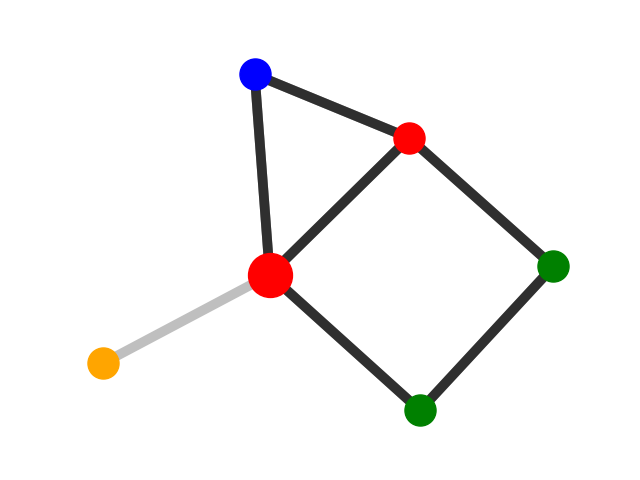
\includegraphics[width=.1\linewidth]{../openreview/imgs/simplification/syn1_pg.png}
& 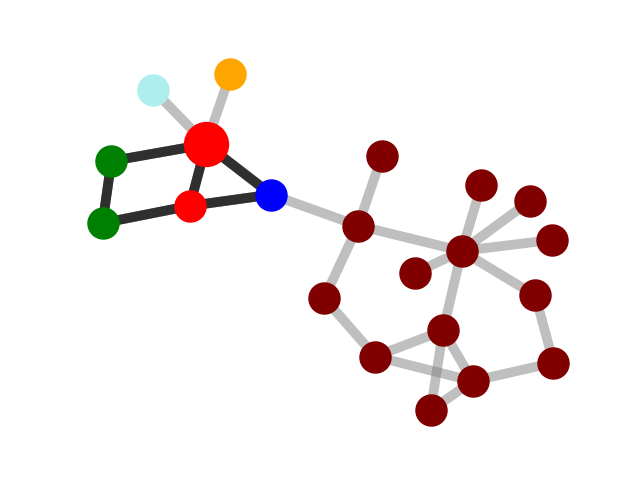
\includegraphics[width=.1\linewidth]{../openreview/imgs/simplification/syn2_pg.png} & 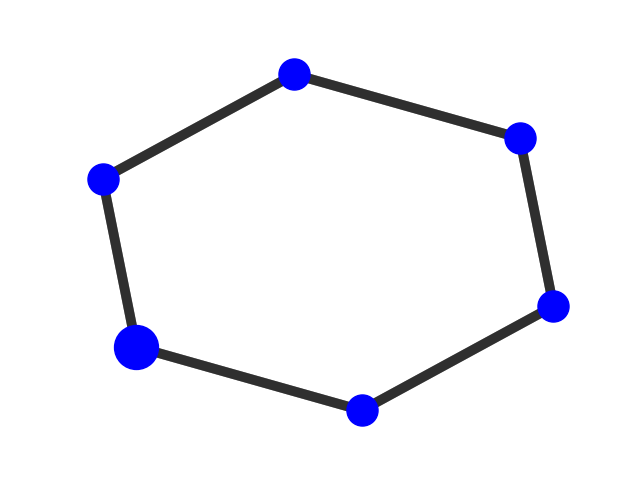
\includegraphics[width=.1\linewidth]{../openreview/imgs/simplification/syn3_pg.png} & \multicolumn{1}{l|}{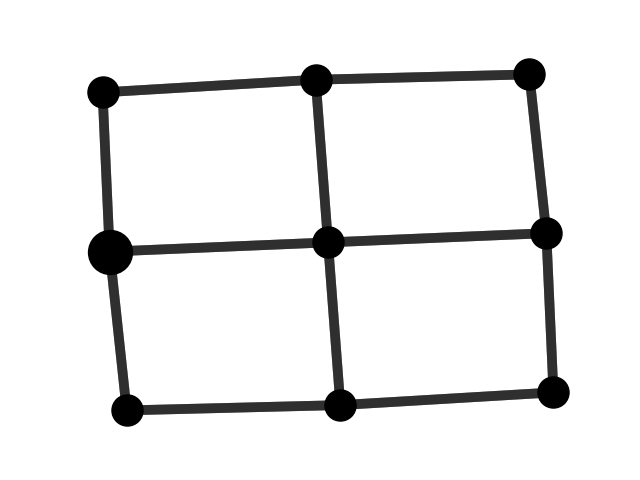
\includegraphics[width=.1\linewidth]{../openreview/imgs/simplification/syn4_pg.png}} & 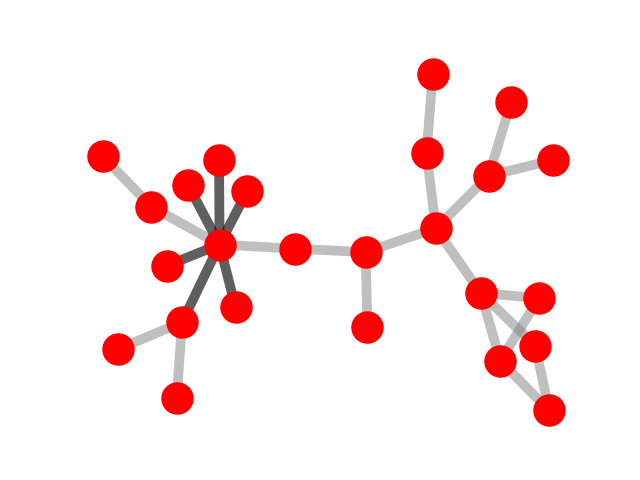
\includegraphics[width=.1\linewidth]{../openreview/imgs/simplification/ba_pg.png} & 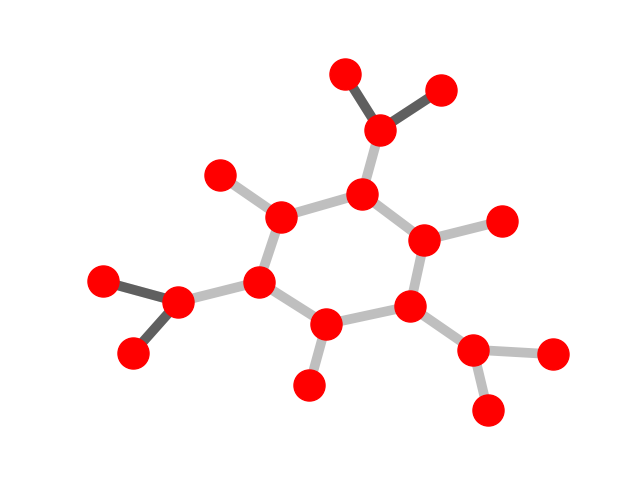
\includegraphics[width=.1\linewidth]{../openreview/imgs/simplification/mutag_pg.png} \\ \hline
GNNExplainer &  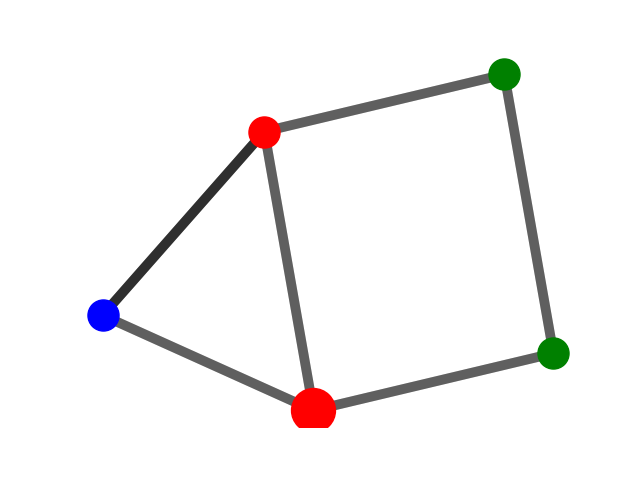
\includegraphics[width=.1\linewidth]{../openreview/imgs/simplification/syn1_gnn.png}
& 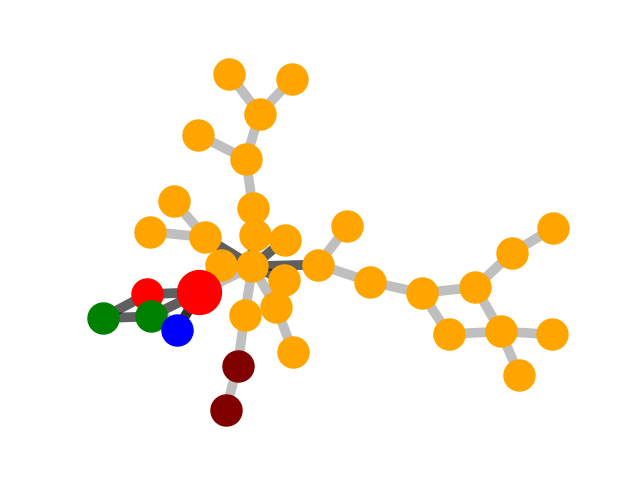
\includegraphics[width=.1\linewidth]{../openreview/imgs/simplification/syn2_gnn.png} & 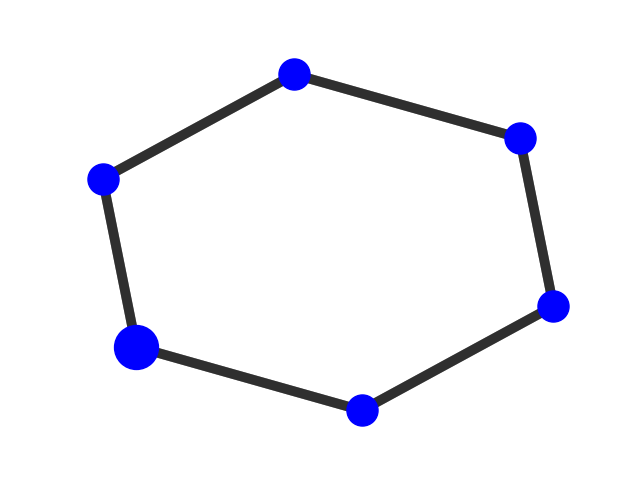
\includegraphics[width=.1\linewidth]{../openreview/imgs/simplification/syn3_gnn.png} & \multicolumn{1}{l|}{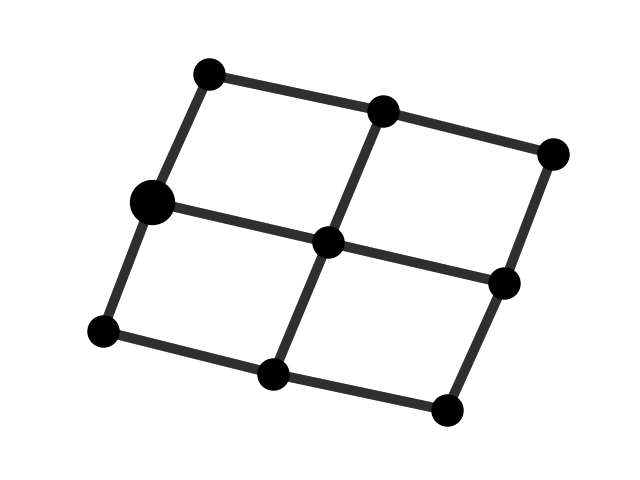
\includegraphics[width=.1\linewidth]{../openreview/imgs/simplification/syn4_gnn.png}} & 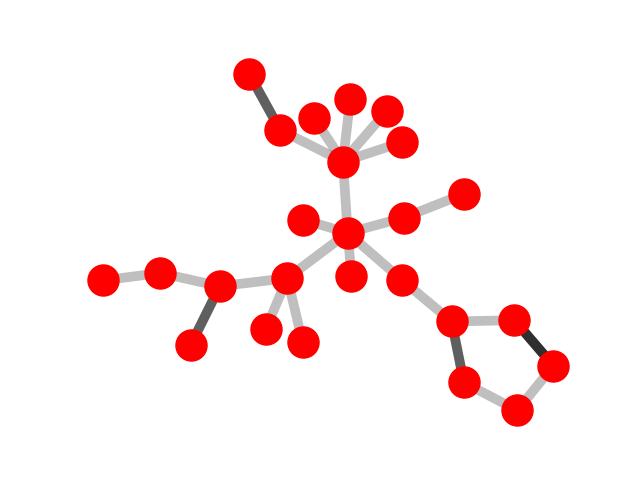
\includegraphics[width=.1\linewidth]{../openreview/imgs/simplification/ba_gnn.png} & 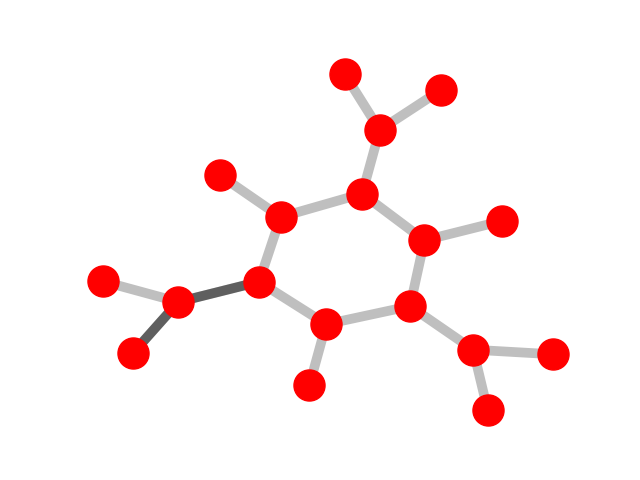
\includegraphics[width=.1\linewidth]{../openreview/imgs/simplification/mutag_gnn.png} \\\hline
\multicolumn{7}{l}{\textbf{Explanation AUC (quantitative}} \\ \hline
Original & 0.963 ± 0.011 & 0.945 ± 0.019 & 0.987 ± 0.007 & \multicolumn{1}{l|}{0.907 ± 0.014} & 0.926 ± 0.021 & 0.873 ± 0.013 \\ 
PGExplainer & 0.999 ± 0.000 & 0.825 ± 0.040 & 0.760 ± 0.014 & \multicolumn{1}{l|}{0.679 ± 0.008} & 0.133 ± 0.046 & 0.843 ± 0.084 \\ 
GNNExplainer & 0.742 ± 0.006 & 0.708 ± 0.004 & 0.540 ± 0.017 & \multicolumn{1}{l|}{0.714 ± 0.002} & 0.499 ± 0.004 & 0.587 ± 0.002 \\ 
Improvement & 34.6\% & 16.5\% & 40.7\% & \multicolumn{1}{l|}{-4.9\%} & -375.2\% & 43.6\% \\ \hline
\multicolumn{7}{l}{\textbf{Inference Time (ms) (efficiency)}} \\ \hline
PGExplainer & 3.58 & 5.23 & 0.45 & \multicolumn{1}{l|}{0.54} & 0.33 & 2.05 \\
GNNExplainer & 58.80 & 91.81 & 52.81 & \multicolumn{1}{l|}{65.54} & 5.21 & 12.32 \\
Speedup & 16x & 17x & 117x & \multicolumn{1}{l|}{121x} & 16x & 6x \\
\bottomrule
\end{tabular}}
\caption{Replicated experimental results from the quantitative, qualitative and efficiency study. The original scores are copied from the paper directly. As the authors of the PGExplainer paper did not report the seeds used for the 10 validation results, we were unable to replicate these results using the authors own codebase. For the qualitative visualization the samples are handpicked similar to the original paper. Node colors represent the node labels (if all colours are the same the nodes are unlabeled). Darkness of the edges signals importance for the final classification decision. In case of the node-classification datasets the bigger node is the one for which the classification is being explained. For the quantitative explanation the average AUC score for the PGExplainer and GNNExplainer and the standard deviation is given. The "original" row reports the PGExplainer AUC score from the original paper. The inference time reported represents the time needed to explain a single sample in milliseconds.}
\label{tab:reproduction_results2}
\end{table}

Quantitatively there is a large difference in the reported AUC scores and what we were able to achieve using the specified configurations for the PGExplainer. Only for BA-Shapes a AUC equal or higher then the presented AUC score was observed. However, BA-Shapes did require some minor modifications to the configurations to get it to work. With the temperature parameter set as originally presented in the code, the evaluation crashed. Only when the temperature was changed to the configuration as presented in the paper we were able to run the evaluation. Similarly, with the configuration as described in the code, the PGExplainer produces the opposite of the expected result for the BA-2Motifs dataset. This is reflected both quantitatively and qualitatively. However, it should be noted that the same drop in AUC score between our implementation and the one originally reported score can also be seen for the GNNExplainer. Due to this, the reported improvement of the PGExplainer over the GNNExplainer remains valid. 

We believe that the difference seen between the AUC scores originally reported for the two explainers and what we observed during our reproduction might be the result of the undocumented effect of the entropy/size regularizations and used temperature. Based on empirical observations we found that the final AUC score is highly dependent on these three hyperparameters. A small follow-up ablation study presented in Tab.\,\ref{tab:reg} confirms this. 

\begin{table}[]
\normalsize
\scalebox{0.80}{
\begin{tabular}{@{}c|l|llllll@{}}
\toprule
\multicolumn{1}{l|}{\textbf{Reg.}} &       & \multicolumn{6}{c}{\textbf{Size}}                                                                \\ \midrule
\multicolumn{1}{l|}{}              &       & 10            & 1             & 0.1           & 0.01        & 0.001       & 0.0001               \\ \midrule
\multirow{5}{*}{\textbf{Entropy}}  & 10    & 0.761 ± 0.014 & 0.761 ± 0.014 & 0.762 ± 0.014 & 0.713 ± 0.156 & 0.628 ± 0.221 & 0.634 ± 0.239          \\
                                  & 1     & 0.761 ± 0.014 & 0.760 ± 0.014   & 0.760 ± 0.015   & 0.683 ± 0.154 & 0.700 ± 0.247 & 0.708 ± 0.226          \\
                                  & 0.1   & 0.761 ± 0.014   & 0.760 ± 0.014   & 0.758 ± 0.015   & 0.565 ± 0.246 & 0.747 ± 0.209 & 0.764 ± 0.214          \\
                                  & 0.01  & 0.761 ± 0.014   & 0.760 ± 0.014   & 0.758 ± 0.015   & 0.551 ± 0.249 & 0.748 ± 0.216 & \textbf{0.776 ± 0.210} \\
                                  & 0.001 & 0.761 ± 0.014   & 0.760 ± 0.014   & 0.758 ± 0.015   & 0.547 ± 0.253 & 0.753 ± 0.216 & 0.763 ± 0.211          \\ \bottomrule
\end{tabular}}
\caption{Results of a small ablation study on the effect of the size and entropy regularization on the AUC score. The ablation study is performed using the Tree-Cycles dataset and follows the setup of the quantitative evaluation. It averages over 10 runs. The results show that the regularization has a large effect on both the quantitative quality of the explanations and their consistency. The best score is shown in bold. }
\label{tab:reg}
\end{table}

\paragraph{Qualitative}
The replicated qualitative evaluation is very similar to the original results. PGExplainer is very capable of finding the motifs in the graphs and highlighting their edges. The same holds for the GNNExplainer. 

The main observed difference is the Mutagenicity dataset. In our replication, only two edges are darkened in contrast to the ten edges darkened in the original paper. However, this difference is created artificially by a difference in the $k$ value reported in the paper and used in the code. While this difference therefore does not tell us anything about the quality of the explanation, it does show the importance of the $k$ hyperparameter. This is further discussed in the Sec.\,\ref{sec6}.

\paragraph{Efficiency}
In terms of efficiency, the reimplemention results are consistent with the claims of the authors. The use of different frameworks between the original implementation and our reimplementation makes a direct comparison of the result is ill advised, but the speedup between the PGExplainer and the GNNExplainer is consistent.